\documentclass{article}
\usepackage{pgfplots}
\pgfplotsset{compat=1.16}

\begin{document}

\begin{figure}[h]
\centering
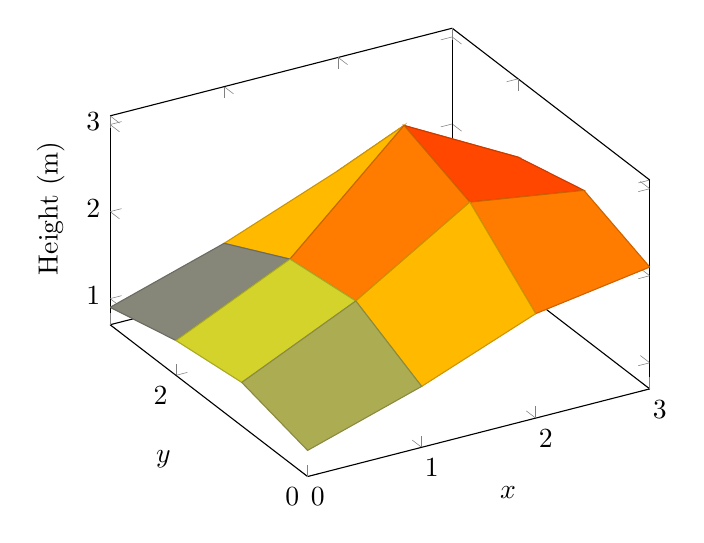
\begin{tikzpicture}
\begin{axis}[
    xlabel=$x$,
    ylabel=$y$,
    zlabel={Height (m)},
    view={-30}{40},
]
\addplot3[surf, mesh/rows=4] table {
x y z
0 0 1.0
1 0 1.4
2 0 1.9
3 0 2.1
0 1 1.2
1 1 1.8
2 1 2.6
3 1 2.4
0 2 1.1
1 2 1.7
2 2 2.9
3 2 2.2
0 3 0.9
1 3 1.3
2 3 1.8
3 3 1.6
};
\end{axis}
\end{tikzpicture}
\caption{Terrain measured on a $4 \times 4$ grid.}
\end{figure}

\end{document}
